\section{Device Optimizations}
\label{sec:deviceoptimization}

Dreslinski et al. \cite{Dreslinski:2010ez} suggest modifications of the transistor structure to reduce delay by reducing inverse sub-threshold slope ($S_S$). 
This can take the form of either modifying the channel doping profile \cite{Paul:2004cx} or increasing oxide length \cite{Hanson:2007uu}.

Hanson shows that the main delay benefit from scaling $S_S$ comes from the assumption that the system voltage is such that the CMOS gate is operating at the minimum energy point, a point far into sub-threshold that is proportional to $S_S$. 
For near-threshold operation, the voltage is instead set by the transistor threshold voltage. 
With the voltage dependence on $S_S$ removed, this equation instead becomes

\begin{equation}
t_p \propto \frac{1}{e^\frac{V_{D}-V_{TH}}{S_S}}
\end{equation} 

which is a much weaker effect considering that $S_S$ in the range of 80-90mV. 

The actual correlation of delay to $S_S$ is even weaker because Hanson is using an equation that assumes we are far sub-threshold. 
As we pass $V_{TH}$, the current and delay begin to instead scale with an interpolation between super-threshold and sub-threshold models rather than just the sub-threshold model. 
Because the super-threshold model doesn't have a reliance on $S_S$, this means that the effect of modifications to $S_S$ on system delay get weaker as voltage moves into the near-threshold regime.

 Raychowdhury \cite{Raychowdhury:2006fu} shows this weakening of $S_S$'s effect on delay in Figure~\ref{fig:doping}
  
\begin{figure}[thpb]
    \centering
    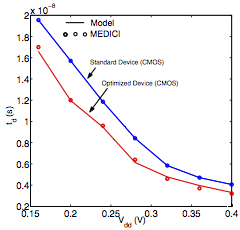
\includegraphics[width=0.4\textwidth]{raychowdhury_doping.png}
    \caption{Effect of sub threshold slope optimization on delay at different voltages.~\cite{Raychowdhury:2006fu}}
    \label{fig:doping}
\end{figure}
 
